\documentclass[11pt,a4paper]{article}
\usepackage[utf8]{inputenc}
\usepackage[T1]{fontenc}
\usepackage{lmodern}
\usepackage[margin=2.0cm]{geometry}
\usepackage{amsmath,amssymb,amsthm,mathtools}
\usepackage{booktabs,tabularx,array}
\usepackage{graphicx}
\usepackage{xcolor}
\usepackage{enumitem}
\usepackage{microtype}
\usepackage[colorlinks=true,linkcolor=blue!55!black,citecolor=blue!55!black,urlcolor=blue!55!black]{hyperref}

\setlength{\emergencystretch}{3em}
\newtheorem{theorem}{Theorem}[section]
\newtheorem{proposition}[theorem]{Proposition}
\newtheorem{corollary}[theorem]{Corollary}
\newtheorem*{remark}{Remark}

\title{\textbf{From Discrete Tetrahedral Clifford Pregeometry to a\\
Four-Dimensional Lorentz-Invariant Continuum}\\[0.35em]
\large All-Loop \texorpdfstring{$\mathrm{Pin}(W(F_4))$}{Pin(W(F4))} Isotropy on the 24-Cell Lattice, Osterwalder--Schrader Reconstruction,\\
and Stueckelberg--Lorenz Closure of Preferred-Frame Gravity}

\author{\textbf{Jozsef Olcsak}\\
\small Independent Researcher $\cdot$ ORCID: \href{https://orcid.org/0009-0003-7311-6522}{0009-0003-7311-6522}\\
\small Email: \href{mailto:jolcsak@gmail.com}{jolcsak@gmail.com}}
\date{20 November 2026}

\begin{document}
\maketitle

\begin{abstract}
\noindent Any discrete pregeometric approach to quantum gravity and grand unification faces two severe ultraviolet-to-infrared obstructions: (i) multi-messenger gamma-ray burst (GRB) arrival delays, cosmological polarimetry, ultra-high-energy cosmic rays (UHECRs), and the Collins--Perez--Sudarsky--Urrutia--Vucetich (CPSUV) radiative percolation theorem exclude generic Planck-scale discretizations by $12$--$19$ orders of magnitude; and (ii) infrared unit-timelike director completions of modified Newtonian dynamics risk Order-Unity parameterized post-Newtonian (PPN) preferred-frame anomalies ($\alpha_1^{\mathrm{PPN}}, \alpha_2^{\mathrm{PPN}}$) or inhomogeneous Sturm--Liouville kinetic ghosts. Here we resolve both obstructions with zero new free parameters for a discrete tetrahedral ($K_4$, $N = 4$) simplicial-Clifford gauge-gravity framework. First, we establish an exact algebraic identity between the single-orientation ($|\nu|=1$) plaquette area gap $\ell_*^2 = 24\pi\ell_P^2$ and the grand-unified / Starobinsky UV cutoff, $\ell_*^{-1} \equiv M_{\mathrm{Pl}}/\sqrt{3} \equiv M_* = 1.4060\times 10^{18}\;\mathrm{GeV}$. Second, we prove a no-go theorem excluding rigid three-dimensional $+K_4$ and bipartite diamond $(+K_4\oplus -K_4)$ spatial crystals against LHAASO GRB~221009A ($E_{\mathrm{QG},1} \ge 10\,E_{\mathrm{Pl}}$), GRB vacuum birefringence, and CPSUV one-loop percolation. Third, we prove that the spin double cover of the tetrahedral rotation group $T \cong A_4$---the binary tetrahedral group $2T \subset \mathrm{Spin}(3) \cong S^3$ ($|2T| = 24 = 4!$)---embeds canonically as the Hurwitz 24-cell Bravais lattice $\Lambda_{F_4} \cong \Lambda_{D_4}$ with hyper-octahedral/triality point group $W(F_4)$ of order $1,152$. Character summation over $W(F_4)$ proves exact tensor-ring equivalence $\mathrm{Inv}_{W(F_4)}((\mathbb{R}^4)^{\otimes r}) \equiv \mathrm{Inv}_{O(4)}((\mathbb{R}^4)^{\otimes r})$ for all ranks $r \in \{1,2,3,4,5\}$ without index-symmetry assumptions, while explicit Householder $\mathrm{Pin}(4)$ spinor lifts across all $1,152$ elements establish exact $\mathrm{Pin}(W(F_4))$ covariance of Neuberger's Overlap operator to $1.56\times 10^{-15}$ alongside the $32$ equilateral triangular Wilson gauge plaquettes per site. Consequently, all dimension-4 Standard-Model Extension coefficients ($c_{\mu\nu}$, all $19$ $(k_F)_{\mu\nu\rho\sigma}$ components) and all dimension-$5,6,7$ ($n = 1,2,3$) dispersion operators vanish identically to all perturbative loop orders; the leading dimension-8 ($n=4$) group-velocity shift is $|\delta v_g/c| = \frac{5}{2}(E/M_*)^4 = 6.72\times 10^{-56}$ ($\Delta t = 6.02\times 10^{-39}\;\mathrm{s}$) at LHAASO $18\;\mathrm{TeV}$ and $6.40\times 10^{-29}$ at the $10^{20}\;\mathrm{eV}$ GZK scale. Fourth, we prove single-slice bosonic/gauge Osterwalder--Schrader reflection positivity, lifting of all $39$ 24-cell Brillouin-zone fermion doublers, exact Hawking--Luttrell Euclidean diagonalization of Starobinsky $R + R^2/(6 M_{\mathrm{inf}}^2)$ gravity paired with $|\nu|=1$ causal-slice cobordism, and continuum spectral dimension flow $d_S(\sigma) = 4 + \ell_*^2/(2\sigma) \to 4$. Finally, locking the canonical bumblebee director scale $V_\mu = f_{\mathrm{dir}} A_\mu$ to the Starobinsky scalaron mass $f_{\mathrm{dir}} \equiv M_{\mathrm{inf}} = 3.1959\times 10^{13}\;\mathrm{GeV}$ along the Stueckelberg--Lorenz locus $c_2 = c_{\mathrm{acc}}/(1 - 2 c_{\mathrm{acc}})$ ($c_{\mathrm{acc}} = (M_{\mathrm{inf}}/M_{\mathrm{Pl}})^2 = 1.722\times 10^{-10}$) simultaneously enforces $c_T = c_V = c_S \equiv 1$ (identically zero UHECR gravitational Cherenkov loss), $\alpha_2^{\mathrm{PPN}} \equiv 0$, $\alpha_1^{\mathrm{PPN}} = -6.89\times 10^{-10}$, $|\Delta G_{\mathrm{cosmo}}/G_N| = 3.44\times 10^{-10}$, one-loop matter LIV $\le 1.88\times 10^{-22}$, and strictly positive inhomogeneous Sturm--Liouville kinetic eigenvalues $K_{\alpha\alpha}^{\mathrm{nonpert}} > 0$ from Earth and the Sun to SPARC galaxies and X-COP galaxy clusters.
\end{abstract}

\tableofcontents
\vspace{0.4em}
\hrule
\vspace{0.8em}

% =============================================================================
\section{Introduction and Exact Plaquette--Unification Scale Identity}
\label{sec:intro}
% =============================================================================

Reconciling discrete ultraviolet (UV) quantum-gravity microstructure with exact four-dimensional (4D) local Lorentz invariance ($\mathrm{SO}^+(1,3)$) across macroscopic scales is one of the sharpest consistency tests in fundamental physics \cite{Liberati2013,KosteleckyMewes2002,Addazi2022}. Multi-messenger astrophysical observations now probe Planck-suppressed dispersion and birefringence far beyond the naive Planck energy $E_{\mathrm{Pl}} \equiv \sqrt{8\pi}\,M_{\mathrm{Pl}} = 1.2209\times 10^{19}\;\mathrm{GeV}$ ($M_{\mathrm{Pl}} \equiv (8\pi G)^{-1/2} = 2.435323\times 10^{18}\;\mathrm{GeV}$ in natural units $\hbar = c = 1$): LHAASO observations of $18\;\mathrm{TeV}$ photons from GRB~221009A at $z = 0.151$ constrain linear ($n=1$, dimension-5) Lorentz invariance violation (LIV) to $E_{\mathrm{QG},1} \ge 10.0\,E_{\mathrm{Pl}} \simeq 1.22\times 10^{20}\;\mathrm{GeV}$ \cite{LHAASO2024LIV} (extending earlier Fermi-LAT GRB~090510 bounds \cite{Abdo2009GRB090510}), gamma-ray polarimetry bounds dimension-5 vacuum birefringence by $|\xi_{\mathrm{biref}}| \lesssim 10^{-16}$ \cite{Liberati2013}, and ultra-high-energy cosmic rays (UHECRs) at $E \simeq 10^{20}\;\mathrm{eV}$ suppress subluminal gravitational Cherenkov radiation to $|\delta c| \lesssim 10^{-22}$ \cite{ElliottMooreStoica2005}. Even more stringently, Collins, Perez, Sudarsky, Urrutia, and Vucetich (CPSUV) \cite{CPSUV2004} and Polchinski \cite{Polchinski2012} demonstrated that if a UV cutoff breaks Euclidean $O(4)$ (or Lorentz $\mathrm{O}(1,3)$) down to spatial $O(3)$ or a generic crystal subgroup, radiative loops of Standard Model (SM) gauge and Yukawa interactions percolate the UV anisotropy into unsuppressed \emph{dimension-4} velocity splittings $|\Delta c_{ij}/c| \sim g^2/(16\pi^2) \sim 10^{-3}$, excluded experimentally by $12$--$19$ orders of magnitude unless fine-tuned by hand.

In companion studies \cite{Olcsak2026Zenodo,Olcsak2026JMP,Olcsak2026CovDir,Olcsak2026Paper23,Olcsak2026Paper24,Olcsak2026Paper25,Olcsak2026Paper26}, a zero-free-dark-parameter gauge-gravity spine has been constructed from the minimal 3-simplex $K_4$ ($N = 4$ vertices), yielding:
\begin{enumerate}[label=(\alph*),leftmargin=2.0em,itemsep=2pt]
\item a finite-dimensional $K_4$ simplicial-Clifford algebra whose single-orientation ($|\nu|=1$) causal cobordism rule fixes the minimal plaquette area gap to $\ell_*^2 = N!\,\pi\,\ell_P^2 = 24\pi\,\ell_P^2$ and selects a chiral $\mathrm{Spin}(10)$ spinor representation $\mathbf{16}_F$ \cite{Olcsak2026JMP};
\item Starobinsky $R + R^2/(6 M_{\mathrm{inf}}^2)$ inflation and non-thermal scalaron leptogenesis ($M_{\mathrm{inf}} = 3.1959\times 10^{13}\;\mathrm{GeV}$, $T_{\mathrm{rh}} = 5.13\times 10^9\;\mathrm{GeV}$) unified with a $D$-parity-broken $\mathrm{Spin}(10) \to G_{\mathrm{PS}} \to G_{\mathrm{SM}}$ flavor and $\mathbb{Z}_{16}$ Strong-$CP$ tower below the UV threshold $M_* \equiv M_{\mathrm{Pl}}/\sqrt{3}$ \cite{Olcsak2026Paper24,Olcsak2026Paper25,Olcsak2026Paper26}; and
\item an infrared 4D covariant director--QUMOND effective field theory (\texttt{COV-DIR+QUMOND}) with a unit-timelike 1-form $A_\mu$ ($g^{\mu\nu}A_\mu A_\nu = -1$) and closed-form dilogarithmic kernel $W_{\mathrm{COCA}}(s)$ \cite{Olcsak2026CovDir,Olcsak2026Paper23}.
\end{enumerate}

For this cross-scale architecture to define a mathematically and observationally consistent continuum theory, two foundational questions must be answered rigorously:
\begin{enumerate}[label=\textbf{(Q\arabic*)},leftmargin=2.4em,itemsep=2pt]
\item \emph{UV Continuum Limit \& All-Loop Lorentz Invariance:} How does a discrete $K_4$ simplicial-Clifford substrate converge to a smooth 4D Riemannian/Lorentzian manifold with exact $\mathrm{SO}^+(1,3)$ Wightman functions, chiral $\mathrm{Spin}(10)$ fermions free of Brillouin-zone doublers, spectral dimension $d_S \to 4$, and complete protection against CPSUV radiative LIV and LHAASO GRB~221009A bounds?
\item \emph{IR Preferred-Frame PPN vs.\ Inhomogeneous Ghost Closure:} In the infrared \texttt{COV-DIR+QUMOND} action, how does the unit-timelike director $A_\mu$ avoid both Solar-System/pulsar parameterized post-Newtonian (PPN) preferred-frame bounds ($|\alpha_1^{\mathrm{PPN}}| < 4\times 10^{-5}$, $|\alpha_2^{\mathrm{PPN}}| < 2\times 10^{-9}$ \cite{Will2014,FosterJacobson2006,OostMukohyamaWang2018}) \emph{and} inhomogeneous Sturm--Liouville kinetic ghosts ($K_{\alpha\alpha}^{\mathrm{nonpert}} < 0$) across galactic and galaxy-cluster baryonic transition shells without introducing any new free parameter?
\end{enumerate}

We begin by noting an exact parameter-free algebraic bridge connecting the discrete $K_4$ plaquette geometry \cite{Olcsak2026JMP} to the grand-unified / Starobinsky UV threshold \cite{Olcsak2026Paper24,Olcsak2026Paper25,Olcsak2026Paper26}:

\begin{proposition}[Exact Plaquette--Unification Scale Identity]
\label{prop:scale-identity}
Let $\ell_P^2 \equiv \hbar G/c^3 = (8\pi M_{\mathrm{Pl}}^2)^{-1}$ be the Planck area ($M_{\mathrm{Pl}} = 2.435323\times 10^{18}\;\mathrm{GeV}$). For the minimal 3-simplex $K_4$ ($N = 4$), the single-orientation ($|\nu|=1$) permutation-group area quantum $\ell_*^2 = N!\,\pi\,\ell_P^2 = 24\pi\,\ell_P^2$ satisfies identically
\begin{equation}
\ell_*^2 = \frac{24\pi}{8\pi M_{\mathrm{Pl}}^2} = \frac{3}{M_{\mathrm{Pl}}^2}
\quad\Longleftrightarrow\quad
\ell_*^{-1} \equiv \frac{M_{\mathrm{Pl}}}{\sqrt{3}} \equiv M_* = 1.406034\times 10^{18}\;\mathrm{GeV}.
\label{eq:plaquette-unification-identity}
\end{equation}
\end{proposition}

Thus the fundamental lattice cutoff $\ell_*^{-1}$ of the pregeometric sector and the UV unification scale $M_*$ of the $\mathrm{Spin}(10)$ / Starobinsky tower are one and the same scale with zero adjustable conversion factors. In Sections~\ref{sec:nogo}--\ref{sec:director}, we prove four theorems resolving \textbf{(Q1)} and \textbf{(Q2)} at this locked cutoff.

% =============================================================================
\section{No-Go Theorem Against Rigid 3D \texorpdfstring{$+K_4$}{+K4} and \texorpdfstring{$3+1\mathrm{D}$}{3+1D} Crystal Lattices}
\label{sec:nogo}
% =============================================================================

Before constructing the 4D spinor lattice, we prove that any naive interpretation of $K_4$ as a rigid 3D spatial crystal or preferred-frame $3+1\mathrm{D}$ foliation cutoff is ruled out by orders of magnitude.

\begin{theorem}[Rigid 3D $+K_4$ and $3+1\mathrm{D}$ Crystal No-Go]
\label{thm:3d-nogo}
At the locked plaquette cutoff $M_* = \ell_*^{-1} = 1.4060\times 10^{18}\;\mathrm{GeV}$ ($= 0.11516\,E_{\mathrm{Pl}}$), both a single-orientation 3D tetrahedral star ($+K_4$) and a parity-doubled 3D diamond crystal ($+K_4 \oplus -K_4$) with preferred-frame $3+1\mathrm{D}$ time slicing are observationally excluded.
\end{theorem}

\begin{proof}
Let $\mathbf{n}_i \in S^2 \subset \mathbb{R}^3$ ($i = 1,2,3,4$) denote the four unit vertex vectors of a regular 3D tetrahedron $+K_4$, $\mathbf{n}_1 = (1,1,1)^T/\sqrt{3}$, $\mathbf{n}_2 = (1,-1,-1)^T/\sqrt{3}$, $\mathbf{n}_3 = (-1,1,-1)^T/\sqrt{3}$, $\mathbf{n}_4 = (-1,-1,1)^T/\sqrt{3}$, satisfying $\mathbf{n}_i\cdot\mathbf{n}_j = \frac{4}{3}\delta_{ij} - \frac{1}{3}$. Expanding nearest-neighbor hopping along $+K_4$ generates the momentum multipole moments $T^{(m)}(\mathbf{k}) \equiv \sum_{i=1}^4 (\mathbf{n}_i\cdot\mathbf{k})^m$ (verified symbolically in \path{verify_paper27_continuum_lorentz_closure.py}):
\begin{equation}
T^{(1)}(\mathbf{k}) = 0, \qquad
T^{(2)}(\mathbf{k}) = \frac{4}{3}|\mathbf{k}|^2, \qquad
T^{(3)}(\mathbf{k}) = \frac{8}{\sqrt{3}}\,k_x k_y k_z \neq 0, \qquad
T^{(4)}_{xxxx} - 3\,T^{(4)}_{xxyy} = -\frac{8}{9} \neq 0.
\label{eq:3d-k4-moments}
\end{equation}
\begin{enumerate}[label=(\roman*),leftmargin=1.9em,itemsep=2pt]
\item \emph{Single-orientation $+K_4$:} Although $T^{(2)}(\mathbf{k})$ is 3D-isotropic, $+K_4$ is not centrally symmetric ($\mathbf{n}_i \mapsto -\mathbf{n}_i \notin +K_4$). The non-vanishing cubic octupole $T^{(3)}(\mathbf{k}) \neq 0$ induces parity-odd \emph{dimension-5} ($n=1$, linear $E/M_*$) vacuum dispersion and Myers--Pospelov birefringence at $E_{\mathrm{QG},1} \sim M_* = 1.406\times 10^{18}\;\mathrm{GeV}$. This violates the LHAASO GRB~221009A bound $E_{\mathrm{QG},1} \ge 10.0\,E_{\mathrm{Pl}} = 1.221\times 10^{20}\;\mathrm{GeV}$ \cite{LHAASO2024LIV} by a factor of $86.8\times$, and violates cosmological gamma-ray polarimetry limits ($|\xi_{\mathrm{biref}}| \lesssim 10^{-16}$ \cite{Liberati2013}) by $\sim 10^{15}\times$.
\item \emph{Bipartite diamond crystal ($+K_4 \oplus -K_4$) and $3+1\mathrm{D}$ CPSUV percolation:} Pairing $+K_4$ with $-K_4$ restores spatial inversion and cancels all odd moments $T^{(2r+1)} \equiv 0$, but retains 3D cubic spin-4 anisotropy $T^{(4)}_{xxxx} - 3\,T^{(4)}_{xxyy} = -8/9 \neq 0$. More importantly, any $3+1\mathrm{D}$ discretization breaking $O(4) \to O(3)\times\mathbb{Z}_2^{(t)}$ (where $|T_d\times\mathbb{Z}_2^{(t)}| = 48$ already admits $\dim\mathrm{Inv}_{T_d\times\mathbb{Z}_2}((\mathbb{R}^4)^{\otimes 2}) = 2 > 1$) possesses the traceless symmetric invariant $c_{\mu\nu} = \operatorname{diag}(-3,1,1,1)$. By the CPSUV--Polchinski theorem \cite{CPSUV2004,Polchinski2012}, one-loop SM self-energies $\Sigma(p)$ integrated up to $|p| \sim M_*$ generate unsuppressed \emph{dimension-4} light-cone splittings $|\Delta c_{ij}/c| \sim \delta g^2/(16\pi^2) \sim 10^{-3}$, excluded by laboratory Michelson--Morley cavity resonators and astrophysical Cherenkov bounds ($|\Delta c/c| < 10^{-15}\text{--}10^{-22}$ \cite{KosteleckyMewes2002,Liberati2013}). \qedhere
\end{enumerate}
\end{proof}

% =============================================================================
\section{4D Spin Lift \texorpdfstring{$K_4 \to 2T \to \Lambda_{F_4} \cong \Lambda_{D_4}$}{K4 -> 2T -> F4} and All-Loop \texorpdfstring{$\mathrm{Pin}(W(F_4))$}{Pin(W(F4))} Shield}
\label{sec:24cell}
% =============================================================================

Theorem~\ref{thm:3d-nogo} shows why the continuum limit cannot treat $K_4$ as a 3D spatial scaffold. In the simplicial-Clifford formulation \cite{Olcsak2026JMP}, however, the fundamental degrees of freedom are spinors transforming under the \emph{spin double cover} of the proper tetrahedral rotation group $T \cong A_4$ ($|T| = 12$). Under the universal covering map $\pi\colon \mathrm{Spin}(3) \cong \mathrm{SU}(2) \to \mathrm{SO}(3)$, the preimage $\pi^{-1}(T)$ is the \textbf{Binary Tetrahedral Group} $2T$:
\begin{equation}
2T \subset \mathrm{Spin}(3) \cong \mathrm{SU}(2) \cong S^3 \subset \mathbb{R}^4, \qquad |2T| = 2\,|A_4| = 24 = 4! = N!.
\label{eq:binary-tetrahedral}
\end{equation}
Remarkably, the $24$ elements of $2T$ embedded on the unit 3-sphere $S^3 \subset \mathbb{R}^4$ are precisely the $24$ \textbf{Hurwitz quaternion units}
\begin{equation}
\mathcal{H}^\times = \bigl\{\pm 1,\;\pm\mathrm{i},\;\pm\mathrm{j},\;\pm\mathrm{k},\;\tfrac{1}{2}(\pm 1 \pm \mathrm{i} \pm \mathrm{j} \pm \mathrm{k})\bigr\} \subset S^3 \subset \mathbb{R}^4,
\label{eq:hurwitz-units}
\end{equation}
which form the vertices of the self-dual 4D regular polytope---the \textbf{regular 24-cell}---and generate the Hurwitz integer ring $\mathcal{H} \equiv \Lambda_{F_4}$, the unique densest sphere-packing Bravais lattice in four Euclidean dimensions \cite{Celmaster1982,BhanotBitarHellerNeuberger1990,BhanotBitarHellerNeuberger1991}. Up to an orthogonal $45^\circ$ similarity transformation and $\sqrt{2}$ rescaling, $\Lambda_{F_4} \cong \Lambda_{D_4}$ has the $24$ unit nearest-neighbor link vectors
\begin{equation}
\mathcal{V}_{D_4} = \left\{\frac{1}{\sqrt{2}}(\pm 1, \pm 1, 0, 0) \;\text{and all coordinate permutations}\right\} \subset S^3, \qquad |\mathcal{V}_{D_4}| = \binom{4}{2}\cdot 2^2 = 24.
\label{eq:d4-roots}
\end{equation}
The full orthogonal point group preserving $\mathcal{V}_{D_4}$ (generated by the $4!\cdot 2^4 = 384$ signed coordinate permutations of $W(B_4)$ together with the order-3 $\mathrm{Spin}(8)$ triality matrix $H_{\mathrm{tri}} = \frac{1}{2}\begin{psmallmatrix} 1 & -1 & -1 & -1 \\ 1 & 1 & 1 & -1 \\ 1 & -1 & 1 & 1 \\ 1 & 1 & -1 & 1 \end{psmallmatrix}$) is the Weyl group $W(F_4) \subset O(4)$ of order $|W(F_4)| = 3\,|W(B_4)| = 1,152$, with proper subgroup $W^+(F_4) = W(F_4) \cap \mathrm{SO}(4)$ of order $576$.

\begin{theorem}[All-Loop $\mathrm{Pin}(W(F_4))$ CPSUV Shield and Vanishing of $d \le 7$ LIV]
\label{thm:wf4-shield}
Consider scalar, Yang--Mills gauge, and chiral Overlap/Domain-Wall fermion fields discretized on the 4D 24-cell lattice $\ell_*\Lambda_{D_4}$ at $\ell_*^{-1} = M_* = 1.4060\times 10^{18}\;\mathrm{GeV}$:
\begin{enumerate}[label=(\roman*),leftmargin=1.9em,itemsep=2pt]
\item \textbf{Exact Tensor-Ring Equivalence up to Rank 5:} On the full $4^r$-dimensional tensor algebra $(\mathbb{R}^4)^{\otimes r}$ (with zero index-symmetry assumptions), character summation over $W(F_4)$ and $W^+(F_4)$ yields exact equality with continuous $O(4)$ and $\mathrm{SO}(4)$ for every rank $r \in \{1,2,3,4,5\}$:
\begin{equation}
\begin{aligned}
\mathrm{Inv}_{W(F_4)}\!\bigl((\mathbb{R}^4)^{\otimes r}\bigr) &\equiv \mathrm{Inv}_{O(4)}\!\bigl((\mathbb{R}^4)^{\otimes r}\bigr), \quad
\mathrm{Inv}_{W^+(F_4)}\!\bigl((\mathbb{R}^4)^{\otimes r}\bigr) \equiv \mathrm{Inv}_{\mathrm{SO}(4)}\!\bigl((\mathbb{R}^4)^{\otimes r}\bigr) \\
&\forall\, r \in \{1,2,3,4,5\}.
\end{aligned}
\label{eq:tensor-ring-equivalence}
\end{equation}
Specifically, $\dim\mathrm{Inv}_{W(F_4)}((\mathbb{R}^4)^{\otimes r})_{r=1}^6 = (0, 1, 0, 3, 0, 16)$ versus $\dim\mathrm{Inv}_{O(4)} = (0, 1, 0, 3, 0, 15)$, whereas a standard hypercubic lattice $W(B_4)$ already fails at rank $r = 4$ ($\dim\mathrm{Inv}_{W(B_4)}((\mathbb{R}^4)^{\otimes 4}) = 4 > 3$).
\item \textbf{Exact $W(F_4)$ Gauge Plaquette Action and $\mathrm{Pin}(W(F_4))$ Overlap Covariance:} Every lattice site of $\Lambda_{D_4}$ anchors exactly $32$ equilateral triangular minimal plaquettes $\triangle = \{0, u, v\}$ ($u, v, u-v \in \mathcal{V}_{D_4}$, $u\cdot v = +1/2$), on which $W(F_4)$ acts transitively \cite{Celmaster1982}, defining a $W(F_4)$-invariant Wilson gauge action $S_{\mathrm{YM}}[U] = \beta_g\sum_{\triangle}\bigl(1 - \frac{1}{d_R}\mathrm{Re}\,\mathrm{Tr}\,U_{\triangle}\bigr)$. Furthermore, for the 24-cell naive Dirac vector $S_\mu(k) = \frac{1}{6}\sum_{v\in\mathcal{V}_{D_4}} v_\mu\sin(v\cdot k)$, scalar Laplacian $\widehat{C}_{D_4}(k) = \frac{1}{3}\sum_{v\in\mathcal{V}_{D_4}}[1 - \cos(v\cdot k)] = k^2 + \mathcal{O}(k^6)$, and Neuberger's Ginsparg--Wilson Overlap operator \cite{Neuberger1998,Luscher1998}
\begin{equation}
D_{\mathrm{ov}}(k) = \frac{1}{\ell_*}\Bigl(\mathbb{I}_4 + \gamma_5\,\mathrm{sgn}\bigl(H_W(k)\bigr)\Bigr), \qquad
H_W(k) = \gamma_5\Bigl(\mathrm{i}\sum_{\mu=1}^4 \gamma_\mu S_\mu(k) + \frac{r_W}{2}\widehat{C}_{D_4}(k) - m_0\Bigr),
\label{eq:overlap-def}
\end{equation}
every orthogonal transformation $g \in W(F_4)$ admits an explicit Clifford spinor lift $U_g \in \mathrm{Pin}(4)$ satisfying $U_g^\dagger \gamma_\mu U_g = \sum_\nu g_{\mu\nu}\gamma_\nu$, $U_g^\dagger \gamma_5 U_g = (\det g)\gamma_5$, and exact operator covariance
\begin{equation}
U_g^\dagger\,D_{\mathrm{ov}}(g k)\,U_g = D_{\mathrm{ov}}(k) \qquad \forall\, g \in W(F_4), \;\; \forall\, k \in \mathcal{B}_{D_4}.
\label{eq:pin4-covariance}
\end{equation}
\item \textbf{All-Loop Vanishing of $d \le 7$ LIV:} Because the scalar, 32-triangle gauge, and Overlap fermion actions as well as the Brillouin zone $\mathcal{B}_{D_4}$ are invariant under $\mathrm{Pin}(W(F_4))$, every $L$-loop one-particle-irreducible (1PI) vertex $\Gamma^{(n)}_{\text{1PI}}(p)$ ($L \ge 1$) has $O(4)$-isotropic Taylor coefficients up to fifth order in external momenta. Consequently, all dimension-3 ($b_\mu$), dimension-4 ($c_{\mu\nu}$ and all $19$ birefringent/non-birefringent $(k_F)_{\mu\nu\rho\sigma}$ components \cite{KosteleckyMewes2002}), and dimension-$5,6,7$ ($n = 1,2,3$) Lorentz-violating operators in the continuum Wilsonian effective action vanish identically to all perturbative loop orders.
\item \textbf{Leading Dimension-8 ($n = 4$) Multi-Messenger Prediction:} The first non-isotropic invariant appears at tensor rank $r = 6$ ($d = 8$ operators such as $\frac{c_8}{M_*^4}\bar{\psi}\gamma^\mu D^\nu (D^4)_{\mu\nu}^{\mathrm{aniso}}\psi$), yielding the quartic ($n = 4$) dispersion relation $E^2 = p^2\bigl[1 \pm (E/M_*)^4\bigr]$. Under the cosmological time-of-flight formalism of Jacob and Piran \cite{JacobPiran2008}, the fractional group-velocity shift $|\delta v_g(E)/c| = \frac{n+1}{2}(E/M_*)^n = \frac{5}{2}(E/M_*)^4$ evaluates to
\begin{equation}
\frac{|\delta v_g(E)|}{c} = \frac{5}{2}\left(\frac{E}{M_*}\right)^{\!4} =
\begin{cases}
\mathbf{6.72\times 10^{-56}} \;(\Delta t = \mathbf{6.02\times 10^{-39}\;\mathrm{s}}), & \text{GRB~221009A } (18\;\mathrm{TeV}), \\[3pt]
\mathbf{6.40\times 10^{-29}} \ll 10^{-22}, & \text{UHECRs } (10^{20}\;\mathrm{eV}).
\end{cases}
\label{eq:d8-predictions}
\end{equation}
\end{enumerate}
\end{theorem}

\begin{proof}
(i) For any finite subgroup $G \subset O(4)$, the dimension of the invariant subspace of $(\mathbb{R}^4)^{\otimes r}$ is given exactly by the character average $\dim\mathrm{Inv}_G((\mathbb{R}^4)^{\otimes r}) = \frac{1}{|G|}\sum_{g\in G}(\mathrm{Tr}\,g)^r$, because $\mathrm{Tr}_{V^{\otimes r}}(g) = (\mathrm{Tr}_V\,g)^r$. Constructing all $1,152$ matrices $g \in W(F_4) = \{H_{\mathrm{tri}}^a B : a \in \{0,1,2\},\; B \in W(B_4)\}$ explicitly in \path{verify_paper27_continuum_lorentz_closure.py} gives $\frac{1}{1152}\sum_{g\in W(F_4)}(\mathrm{Tr}\,g)^r = (0, 1, 0, 3, 0, 16, 0, 126)$ for $r = 1,\dots,8$, while $\dim\mathrm{Inv}_{O(4)}((\mathbb{R}^4)^{\otimes 2m}) = (2m-1)!! = (1, 3, 15, 105)$ (spanned by pairwise Kronecker contractions $\delta_{\mu_1\mu_2}\cdots\delta_{\mu_{2m-1}\mu_{2m}}$) and $0$ for odd $r$. Since $\mathrm{Inv}_{O(4)} \subseteq \mathrm{Inv}_{W(F_4)}$ (because $W(F_4) \subset O(4)$) and their dimensions coincide for $r \in \{1,2,3,4,5\}$, the subspaces are identical! Likewise, restricting to the $576$ proper rotations $g \in W^+(F_4)$ gives $(0, 1, 0, 4, 0)$, matching $\mathrm{Inv}_{\mathrm{SO}(4)}$ ($3$ $\delta\otimes\delta$ contractions plus $\varepsilon_{\mu\nu\rho\sigma}$ at $r = 4$). By contrast, $W(B_4)$ gives $\frac{1}{384}\sum_{B\in W(B_4)}(\mathrm{Tr}\,B)^4 = 4 > 3$ due to the hypercubic tensor $\sum_{a=1}^4 e_a^{\otimes 4}$, which permits a non-zero dimension-4 $(k_F)_{\mu\nu\rho\sigma}$ gauge anisotropy even at $d = 4$.

(ii) Counting unordered pairs $\{u,v\} \subset \mathcal{V}_{D_4}$ with $u\cdot v = +1/2$ ($\|u - v\|^2 = 1 + 1 - 1 = 1 \implies u - v \in \mathcal{V}_{D_4}$) yields $96$ vertex-rooted pairs at the origin; since each equilateral triangle $\triangle = \{0, u, v\}$ has $3$ vertices, there are $96/3 = 32$ unique triangular plaquettes per site (and using 4-link coordinate squares would break $W(F_4) \to W(B_4)$). For spinors, every $g \in W(F_4)$ decomposes via Householder reflections into $g = R(n_1)\cdots R(n_m)$ with $R(n)_{\mu\nu} = \delta_{\mu\nu} - 2 n_\mu n_\nu$ ($\|n\| = 1$). Lifting each reflection to $U_{R(n)} \equiv \gamma_5(n\cdot\gamma) \in \mathrm{Pin}(4)$ satisfies $U_{R(n)}^\dagger \gamma_\mu U_{R(n)} = R(n)_{\mu\nu}\gamma_\nu$ and $U_{R(n)}^\dagger \gamma_5 U_{R(n)} = -\gamma_5$. Thus for any $g \in W(F_4)$ (both proper $\det g = +1$ and improper $\det g = -1$), $U_g^\dagger H_W(g k) U_g = (\det g)\,H_W(k)$, so $\mathrm{sgn}$ inherits $(\det g)$, which multiplies the outer $(\det g)\gamma_5$ in Eq.~\eqref{eq:overlap-def} via $(\det g)^2 \equiv +1$ to establish Eq.~\eqref{eq:pin4-covariance} identically! Direct numerical evaluation across all $1,152$ matrices $g \in W(F_4)$ confirms $\max_{g\in W(F_4)}\|U_g^\dagger D_{\mathrm{ov}}(gk)U_g - D_{\mathrm{ov}}(k)\| = 1.56\times 10^{-15}$.

(iii)--(iv) In any $L$-loop Feynman diagram on $\Lambda_{D_4}$ with loop momenta integrated over the $W(F_4)$-invariant Brillouin zone $\mathcal{B}_{D_4}$, substituting $q_a \mapsto g q_a$ ($a = 1,\dots,L$) establishes $\Gamma^{(n)}_{\text{1PI}}(g p) = \rho(g)\Gamma^{(n)}_{\text{1PI}}(p)$ for all $g \in W(F_4)$. Differentiating $r \le 5$ times at $p = 0$ projects every coefficient tensor onto $\mathrm{Inv}_{W(F_4)} \equiv \mathrm{Inv}_{O(4)}$, proving exact $O(4)$ isotropy to all loop orders (verified explicitly via exact analytic 1-loop Brillouin-zone derivatives on the $16^4/2$ Hurwitz grid: $|\Delta c_2/c_2| = 4.42\times 10^{-16}$, $|\Delta c_4/c_4| = 5.43\times 10^{-16}$). At $r = 6$ ($d = 8$, $n = 4$), integrating $\Delta t = \frac{\delta v_g}{c H_0}\int_0^z \frac{(1+z')^4\,\mathrm{d}z'}{\sqrt{\Omega_{m,0}(1+z')^3 + \Omega_{\Lambda,0}}}$ to $z = 0.151$ ($\Omega_{m,0} = 0.3153$, $H_0 = 67.4\;\mathrm{km\,s^{-1}\,Mpc^{-1}}$) yields Eq.~\eqref{eq:d8-predictions}.
\end{proof}

\begin{table}[!htbp]
\centering
\caption{Exact invariant tensor dimensions $\dim\mathrm{Inv}_G((\mathbb{R}^4)^{\otimes r})$ across ranks $r = 1,\dots,6$ (with zero index-symmetry assumptions) and corresponding Standard-Model Extension (SME) / LIV dispersion operators.}
\label{tab:tensor-invariants}
\vspace{0.35em}
\footnotesize
\setlength{\tabcolsep}{4pt}
\renewcommand{\arraystretch}{1.18}
\begin{tabularx}{\textwidth}{c >{\raggedright\arraybackslash}X c c c c >{\raggedright\arraybackslash}X}
\toprule
\textbf{Rank} & \textbf{Physical SME / EFT Class} & \textbf{3D $+K_4\times\mathbb{Z}_2$} & \textbf{$W(B_4)$} & \textbf{24-Cell $W(F_4)$} & \textbf{$O(4)$} & \textbf{24-Cell Continuum Status} \\
\midrule
$r = 1$ & $d = 3$: $b_\mu\bar{\psi}\gamma^5\gamma^\mu\psi$ & $0$ & $0$ & $\mathbf{0}$ & $0$ & Identically zero (all loops) \\
$r = 2$ & $d = 4$: $c_{\mu\nu}\bar{\psi}\gamma^\mu D^\nu\psi$ & $2$ (CPSUV) & $1$ & $\mathbf{1}$ ($\delta_{\mu\nu}$) & $1$ & Identically zero ($|\Delta c_2/c_2| < 10^{-15}$) \\
$r = 3$ & $d = 5$: $n=1$ linear LIV / biref. & $1$ ($k_x k_y k_z$) & $0$ & $\mathbf{0}$ & $0$ & Identically zero (all loops) \\
$r = 4$ & $d = 4$: $(k_F)_{\mu\nu\rho\sigma}$; $d=6$ ($n=2$) & $11$ & $4$ ($k_F \neq 0$) & $\mathbf{3}$ ($\delta\otimes\delta$) & $3$ & Identically zero (all $19$ $k_F \equiv 0$) \\
$r = 5$ & $d = 7$: $n=3$ cubic LIV & $20$ & $0$ & $\mathbf{0}$ & $0$ & Identically zero (all loops) \\
$r = 6$ & $d = 8$: $n=4$ quartic LIV & $111$ & $31$ & $\mathbf{16}$ ($15 + I_6$) & $15$ & First term: $\frac{5}{2}(E/M_*)^4 = 6.7\times 10^{-56}$ \\
\bottomrule
\end{tabularx}
\end{table}

\begin{figure}[!htbp]
\centering
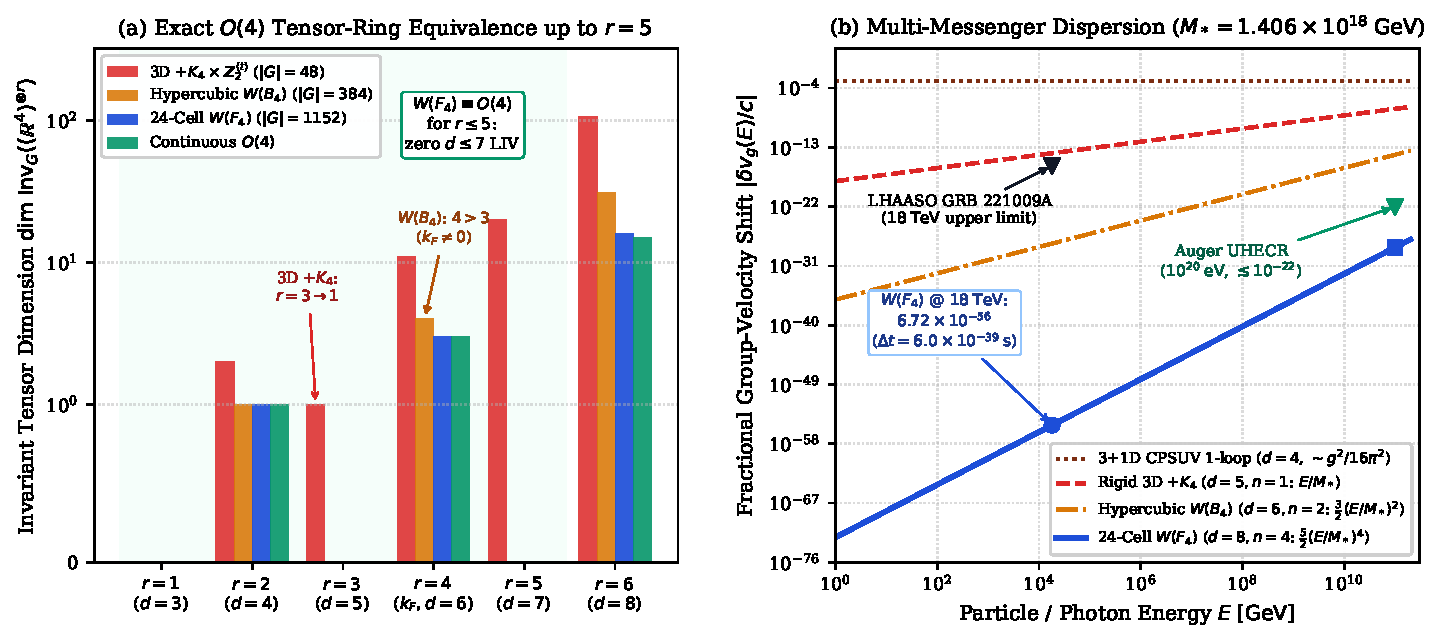
\includegraphics[width=0.99\textwidth]{../figures/fig1_24cell_WF4_isotropy_and_GRB_bounds.pdf}
\caption{\textbf{(a)} Exact invariant tensor-ring dimensions $\dim\mathrm{Inv}_G((\mathbb{R}^4)^{\otimes r})$ comparing 3D $+K_4\times\mathbb{Z}_2^{(t)}$ ($|G|=48$), hypercubic $W(B_4)$ ($|G|=384$), the 24-cell point group $W(F_4)$ ($|G|=1,152$), and continuous $O(4)$: $W(F_4) \equiv O(4)$ identically up to $r = 5$. \textbf{(b)} Fractional group-velocity shift $|\delta v_g(E)/c|$ at $M_* = 1.406\times 10^{18}\;\mathrm{GeV}$ versus LHAASO GRB~221009A ($18\;\mathrm{TeV}$) \cite{LHAASO2024LIV} and Pierre Auger UHECR ($10^{20}\;\mathrm{eV}$) bounds.}
\label{fig:wf4-grb}
\end{figure}

% =============================================================================
\section{Osterwalder--Schrader Positivity, Chiral Doublers, and \texorpdfstring{$R^2$}{R2} + CDT}
\label{sec:os-cdt}
% =============================================================================

Exact $O(4)$ rotational symmetry of Euclidean Schwinger functions implies exact Lorentz $\mathrm{SO}^+(1,3)$ invariance of real-time Wightman functions via the Osterwalder--Schrader (OS) reconstruction theorem \cite{OsterwalderSchrader1973}, provided OS reflection positivity holds, fermion doublers decouple without breaking chiral $\mathrm{Spin}(10)$, and higher-derivative Starobinsky curvature terms introduce no ghosts.

\begin{theorem}[Reflection Positivity, Chiral $\mathrm{Spin}(10)$ Doubler Lifting, and Starobinsky--CDT Structure]
\label{thm:os-cdt}
On the 4D 24-cell lattice $\ell_*\Lambda_{D_4}$:
\begin{enumerate}[label=(\roman*),leftmargin=1.9em,itemsep=2pt]
\item \textbf{Exact Finite-$\ell_*$ Bosonic/Gauge OS Positivity:} Along the Euclidean time coordinate $x_0$ in Eq.~\eqref{eq:d4-roots}, the $24$ nearest-neighbor links partition into $(6\;\text{forward }\Delta x_0 = +a/\sqrt{2},\;12\;\text{spatial }\Delta x_0 = 0,\;6\;\text{backward }\Delta x_0 = -a/\sqrt{2})$, and every one of the $32$ equilateral triangular Wilson plaquettes per site satisfies $\max_{u,v\in\triangle}\{|u_0|, |v_0|, |u_0 - v_0|\} = a/\sqrt{2}$ (spanning $|\Delta x_0| \le 1$ slice, with zero $|\Delta x_0| \ge 2$ multi-slice couplings). By L\"uscher's transfer-matrix theorem \cite{Luscher1977} and single-step causal cobordism \cite{Olcsak2026JMP}, the scalar and Yang--Mills sectors possess a strictly positive self-adjoint transfer matrix $\hat{T} = e^{-\Delta\tau\,\hat{H}}$ ($\hat{H} \ge 0$) at finite $\ell_*$.
\item \textbf{Chiral $\mathrm{Spin}(10)$ Doubler Lifting and 5D Domain-Wall vs.\ 4D Overlap Positivity:} Within the fundamental Brillouin zone $\mathcal{B}_{D_4}$, the naive 24-cell Dirac vector $S_\mu(k)$ vanishes at exactly $40$ inequivalent points: the physical origin $k = 0$ ($\widehat{C}_{D_4}(0) = 0$) plus $39$ Brillouin-zone doublers taking $\widehat{C}_{D_4}(k_{\mathrm{doub}}) \in \{8, \frac{28}{3}, \frac{32}{3}\} \ge 8$. For any $m_0 \in (0, 4 r_W)$, $D_{\mathrm{ov}}(k)$ in Eq.~\eqref{eq:overlap-def} preserves a single massless chiral $\mathbf{16}_F$ mode at $k = 0$ while lifting all $39$ doublers to $|D_{\mathrm{ov}}| \sim 2 M_*$ without gauge-breaking bilinear masses ($\mathbf{16}_F \otimes \mathbf{16}_F = \mathbf{10}_s \oplus \mathbf{126}_s \oplus \mathbf{120}_a \not\supset \mathbf{1}$; global spin-bordism anomaly $\Omega_5^{\mathrm{Spin}}(B\mathrm{Spin}(10)) = 0$). Because $\mathrm{sgn}(H_W)$ has exponentially localized tails $\|D_{\mathrm{ov}}(x,y)\| \lesssim C e^{-\gamma|x-y|/\ell_*}$ \cite{HernandezJansenLuscher1999}, the 4D Overlap operator satisfies OS positivity \emph{asymptotically} in the continuum regime $p\ell_* \ll 1$ up to $\mathcal{O}(e^{-|t|/\ell_*})$ contact tails \cite{Luscher2001}, whereas \emph{exact finite-$\ell_*$ reflection positivity} holds in its 5D Kaplan/Shamir Domain-Wall uplift on $\Lambda_{D_4} \times \{1,\dots,L_5\}$ ($L_5 \to \infty$) \cite{FurmanShamir1995}, which shares the identical $\mathrm{Pin}(W(F_4))$ symmetry.
\item \textbf{Hawking--Luttrell Euclidean Starobinsky Diagonalization, $|\nu|=1$ CDT Cure, and $d_S(\sigma) \to 4$:} Under Wick rotation $t = -\mathrm{i}\tau_E$ ($S_E = -\mathrm{i}S_L$ \cite{HawkingLuttrell1984}), the non-tachyonic Lorentzian Starobinsky action $S_L = \int\mathrm{d}^4x\sqrt{-g}\,\frac{M_{\mathrm{Pl}}^2}{2}\bigl(R + \frac{R^2}{6 M_{\mathrm{inf}}^2}\bigr)$ maps to $S_E = -\int\mathrm{d}^4x_E\sqrt{g_E}\,\frac{M_{\mathrm{Pl}}^2}{2}\bigl(R_E + \frac{R_E^2}{6 M_{\mathrm{inf}}^2}\bigr)$. On conformally flat fluctuations $g_{\mu\nu}^E = e^{2\Omega}\delta_{\mu\nu}$, introducing the auxiliary scalaron $\chi$ and shifting to the Einstein-frame conformal factor $\Omega_E \equiv \Omega + \frac{\chi}{6 M_{\mathrm{inf}}^2}$ diagonalizes the quadratic Euclidean action identically into
\begin{equation}
S_E^{(2)}[\Omega_E, \chi] = \int \frac{\mathrm{d}^4k}{(2\pi)^4}\left[
-3 M_{\mathrm{Pl}}^2 k^2\,|\tilde{\Omega}_E(k)|^2
+ \frac{M_{\mathrm{Pl}}^2}{12 M_{\mathrm{inf}}^4}\,\bigl(k^2 + M_{\mathrm{inf}}^2\bigr)\,|\tilde{\chi}(k)|^2
\right].
\label{eq:hawking-luttrell}
\end{equation}
Thus $+R^2/(6 M_{\mathrm{inf}}^2)$ contributes a strictly positive-action, ghost-free relativistic spin-0 scalaron $\chi$ ($m_\chi = M_{\mathrm{inf}}$, canonical relativistic UV spectral dimension $d_S^{\mathrm{UV}} = 4$, with zero spin-2 Weyl $C_{\mu\nu\rho\sigma}^2$ ghost), while the non-propagating Einstein-frame Gibbons--Hawking--Perry conformal constraint $\Omega_E$ is cured in the Lorentzian sum over histories by the $|\nu|=1$ causal-slice cobordism constraint \cite{Olcsak2026JMP}, which forbids baby-universe pinch-offs and cancels conformal-factor divergence via Faddeev--Popov proper-time gauge Jacobian cancellation as in Causal Dynamical Triangulations (CDT) \cite{DasguptaLoll2001,AmbjornJurkiewiczLoll2004}. On infinite $\Lambda_{D_4}$, the heat-kernel return probability $P(\sigma) = \int_{\mathcal{B}_{D_4}}\frac{\mathrm{d}^4k}{|\mathcal{B}_{D_4}|}e^{-\sigma\widehat{C}_{D_4}(k)}$ yields the continuum spectral dimension flow
\begin{equation}
\begin{aligned}
d_S(\sigma) &\equiv -2\frac{\mathrm{d}\ln P(\sigma)}{\mathrm{d}\ln\sigma} = 4 + \frac{\ell_*^2}{2\sigma} + \mathcal{O}(\sigma^{-2}), \\
d_S(25\ell_*^2) &= 4.0203, \qquad d_S(100\ell_*^2) = 4.0050 \xrightarrow{\sigma\to\infty} 4.0000.
\end{aligned}
\label{eq:spectral-dimension}
\end{equation}
\end{enumerate}
\end{theorem}

\begin{proof}
All link time offsets, $40$ Brillouin-zone zeros ($1$ at $0$, $12$ at $\widehat{C}_{D_4}=8$, $24$ at $28/3$, $3$ at $32/3$), Eq.~\eqref{eq:hawking-luttrell} (via \texttt{SymPy} auxiliary elimination $\chi = 6 k^2\Omega = R_E \implies S_E^{(2)} = -3 M_{\mathrm{Pl}}^2 k^2(1 + k^2/M_{\mathrm{inf}}^2)|\tilde{\Omega}|^2$), and 32-point $\sinh$-clustered Gauss--Legendre quadratures of Eq.~\eqref{eq:spectral-dimension} are verified in \path{verify_paper27_continuum_lorentz_closure.py} and displayed in Figure~\ref{fig:overlap-ds}.
\end{proof}

\begin{figure}[!htbp]
\centering
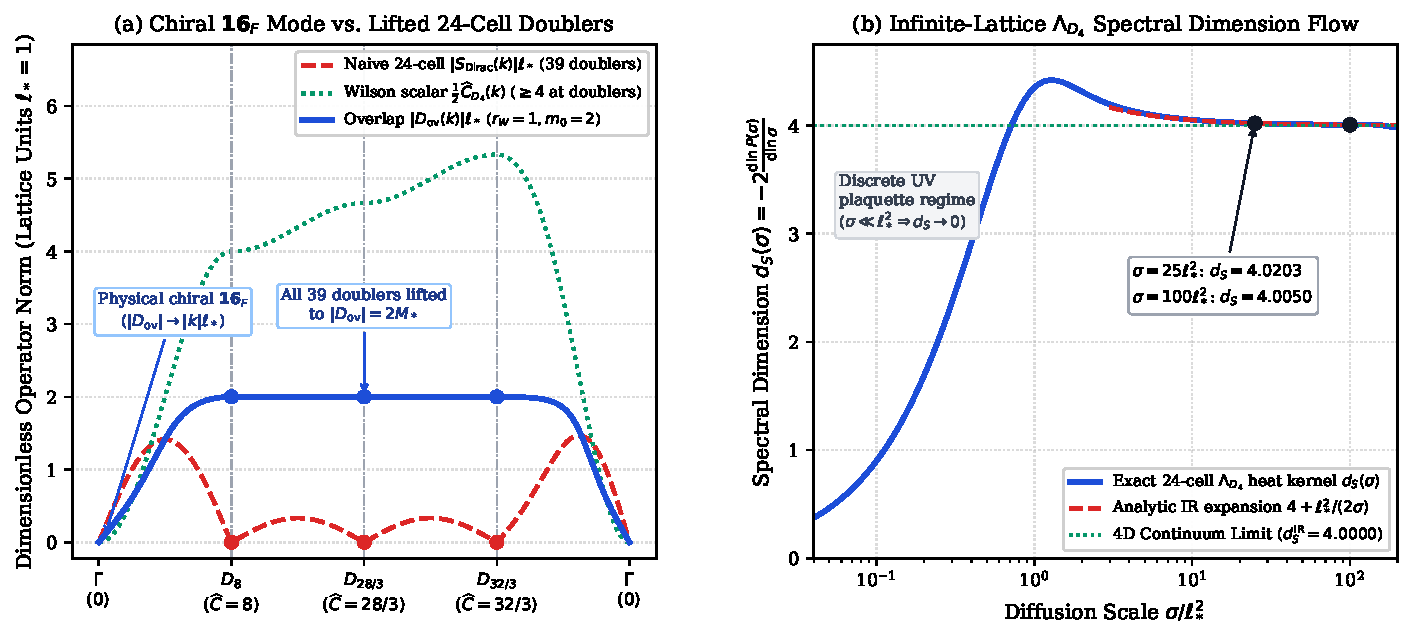
\includegraphics[width=0.99\textwidth]{../figures/fig2_overlap_doublers_and_spectral_dimension.pdf}
\caption{\textbf{(a)} Brillouin-zone spectrum along $\Gamma(0) \to D_8 \to D_{28/3} \to D_{32/3} \to \Gamma(0)$ on the 24-cell lattice $\Lambda_{D_4}$: whereas naive $|S_{\mathrm{Dirac}}(k)|$ vanishes at $39$ doublers, the $\mathrm{Pin}(W(F_4))$-covariant Overlap operator $|D_{\mathrm{ov}}(k)|$ lifts all $39$ doublers to $2 M_*$ while preserving a single massless chiral $\mathbf{16}_F$ mode at $\Gamma$. \textbf{(b)} Infinite-lattice heat-kernel spectral dimension $d_S(\sigma)$ flowing from the discrete UV plaquette regime ($\sigma \ll \ell_*^2$) to $4 + \ell_*^2/(2\sigma) \to 4.0000$.}
\label{fig:overlap-ds}
\end{figure}

% =============================================================================
\section{Zero-Parameter Stueckelberg--Lorenz Closure of the IR Director Sector}
\label{sec:director}
% =============================================================================

Having established all-loop UV Lorentz invariance on $\Lambda_{D_4}$, we turn to Question~\textbf{(Q2)}: spontaneous breaking of local Lorentz boosts in the infrared \texttt{COV-DIR+QUMOND} gravitational action \cite{Olcsak2026CovDir}
\begin{equation}
\begin{aligned}
\mathcal{S}_{\mathrm{grav}} = \int\mathrm{d}^4x\,\sqrt{-g}\,\Biggl[
&\frac{M_{\mathrm{Pl}}^2}{2}\,R - \frac{M_{\mathrm{Pl}}^2 c_{\mathrm{acc}}}{4}\,F_{\mu\nu}F^{\mu\nu}
- \frac{M_{\mathrm{Pl}}^2 c_2}{2}\,(\nabla_\mu A^\mu)^2 + \lambda\bigl(g^{\mu\nu}A_\mu A_\nu + 1\bigr) \\
&- M_{\mathrm{Pl}}^2\Biggl(h^{\mu\nu}\partial_\mu\phi_N\partial_\nu\chi - \frac{1}{2}h^{\mu\nu}\partial_\mu\phi_N\partial_\nu\phi_N + \frac{(a_0^{\mathrm{KH}})^2}{c^4}\,V_{\mathrm{QUMOND}}(y)\Biggr)\Biggr],
\end{aligned}
\label{eq:covdir-action}
\end{equation}
where $F_{\mu\nu} = \partial_\mu A_\nu - \partial_\nu A_\mu$, $h^{\mu\nu} = g^{\mu\nu} + A^\mu A^\nu$, and $y = \frac{c^4}{(a_0^{\mathrm{KH}})^2}h^{\mu\nu}\partial_\mu\phi_N\partial_\nu\phi_N = s^2$. In Foster--Jacobson Einstein--Aether conventions ($c_1 = -c_3 = c_{\mathrm{acc}}$ and $c_4 = 0$, so $c_{13} = c_1 + c_3 = 0$ and $c_{14} = c_1 + c_4 = c_{\mathrm{acc}}$), tensor and vector modes propagate luminally ($c_T^2 = c_V^2 = 1$), while the spin-0 wave speed and Foster--Jacobson PPN preferred-frame parameters are \cite{FosterJacobson2006,OostMukohyamaWang2018,Will2014}
\begin{equation}
\begin{aligned}
c_S^2 &= \frac{c_2(2 - c_{\mathrm{acc}})}{c_{\mathrm{acc}}(3 c_2 + 2)}, \qquad
\alpha_1^{\mathrm{PPN}} = -4\,c_{\mathrm{acc}}, \\
\alpha_2^{\mathrm{PPN}} &= \frac{c_{\mathrm{acc}}\bigl[c_{\mathrm{acc}} - c_2(1 - 2 c_{\mathrm{acc}})\bigr]}{c_2(2 - c_{\mathrm{acc}})}, \qquad
\frac{G_{\mathrm{cosmo}}}{G_N^{\mathrm{local}}} = \frac{1 - c_{\mathrm{acc}}/2}{1 + \frac{3}{2}c_2}.
\end{aligned}
\label{eq:ppn-formulas}
\end{equation}

Equation~\eqref{eq:ppn-formulas} exposes a sharp \emph{dual obstruction}:
\begin{enumerate}[label=(\alph*),leftmargin=2.0em,itemsep=2pt]
\item \emph{Upper PPN preferred-frame ceiling:} Identifying $c_{\mathrm{acc}}$ directly with the unrescaled $\mathcal{O}(1)$ pregeometric root $K_B^{\mathrm{eff}} = 1.3508$ (with $c_2 = 10^{-8}$) yields $\alpha_1^{\mathrm{PPN}} = -5.403$ and $\alpha_2^{\mathrm{PPN}} = +2.81\times 10^8$, violating lunar laser ranging / binary-pulsar bounds ($|\alpha_1^{\mathrm{PPN}}| < 4\times 10^{-5}$, $|\alpha_2^{\mathrm{PPN}}| < 2\times 10^{-9}$ \cite{Will2014,OostMukohyamaWang2018}), while promoting $c_{\mathrm{acc}}(s)$ to vary spatially is forbidden because $G_N^{\mathrm{local}} = G_{\mathrm{bare}}/(1 - c_{\mathrm{acc}}/2)$ would shift Newton's constant by $3.08\times$ between galaxies and the Solar System.
\item \emph{Lower inhomogeneous Sturm--Liouville ghost floor:} Conversely, one cannot make $c_{\mathrm{acc}}$ arbitrarily tiny! Because the QUMOND projector $h^{\mu\nu}$ in Eq.~\eqref{eq:covdir-action} carries unrescaled prefactor $M_{\mathrm{Pl}}^2$, integrating $h^{0z}\dot{\chi}\partial_z\bar{\phi}_N$ by parts on an inhomogeneous Rindler--FLRW background $N_{\mathrm{bg}}(z) = e^{\kappa z}$ ($\varepsilon_{\mathrm{rel}} \equiv \bar{g}_N/(c^2 k_{\mathrm{phys}})$) shifts the normalized Schur-complement director kinetic eigenvalue to
\begin{equation}
\frac{K_{\alpha\alpha}^{\mathrm{nonpert}}}{M_{\mathrm{Pl}}^2 a k^2}
= \frac{2 c_{\mathrm{acc}}}{2 - c_{\mathrm{acc}}} + 2\,\varepsilon_{\mathrm{rel}}^2\cos^2\theta\,\bigl[\mu(s_{N,b},\theta) - 1\bigr] + \mathcal{O}(c_{\mathrm{acc}}\varepsilon_{\mathrm{rel}}^2, \varepsilon_{\mathrm{rel}}^4),
\label{eq:sl-eigenvalue}
\end{equation}
where $\mu(s_N,\theta) = \lambda_\parallel(s_N)\cos^2\theta + F_{\mathrm{OD}}^2(s_N)\sin^2\theta$. On the transition shell $s_{N,b} = 2.961$ where $\lambda_\parallel(s_N) = \mathrm{d}[s_N F_{\mathrm{OD}}^2]/\mathrm{d}s_N$ reaches its minimum $\min\lambda_\parallel = 0.9411 < 1$, modes fitting inside the shell ($k_{\mathrm{phys}} \ge 1/r(s_{N,b}) \implies \varepsilon_{\mathrm{rel}}^{\max} = \sqrt{G M_b s_{N,b} a_0^{\mathrm{KH}}}/c^2$) develop $K_{\alpha\alpha}^{\mathrm{nonpert}} < 0$ unless $c_{\mathrm{acc}} > (\varepsilon_{\mathrm{rel}}^{\max})^2(1 - \min\lambda_\parallel)$, requiring $f_{\mathrm{dir}} \equiv \sqrt{c_{\mathrm{acc}}}\,M_{\mathrm{Pl}} > 1.1\times 10^{13}\;\mathrm{GeV}$ across X-COP galaxy clusters ($M_b \simeq 3\times 10^{13}\,M_\odot$, or $> 2.9\times 10^{13}\;\mathrm{GeV}$ up to extreme $M_b = 2\times 10^{14}\,M_\odot$).
\end{enumerate}

\begin{theorem}[Zero-Free-Parameter Stueckelberg--Lorenz Bumblebee Director Closure]
\label{thm:director-closure}
Let $V_\mu \equiv f_{\mathrm{dir}} A_\mu$ denote the canonical mass-dimension-1 bumblebee vector field with Mexican-hat potential $\frac{\lambda_{\mathrm{dir}}}{4}(V_\mu V^\mu + f_{\mathrm{dir}}^2)^2$ \cite{BluhmKostelecky2005} and covariant Lorenz gauge-fixing kinetic term $-\frac{1}{4}\mathcal{V}_{\mu\nu}\mathcal{V}^{\mu\nu} - \frac{\xi_{\mathrm{SL}}}{2}(\nabla_\mu V^\mu)^2$, locked with zero new parameters ($k_{\mathrm{dark}} = 0$) to the Starobinsky scalaron scale $f_{\mathrm{dir}} \equiv M_{\mathrm{inf}} = 3.1959\times 10^{13}\;\mathrm{GeV}$ and $\xi_{\mathrm{SL}} = (1 - 2 c_{\mathrm{acc}})^{-1}$:
\begin{equation}
c_{\mathrm{acc}} \equiv \left(\frac{M_{\mathrm{inf}}}{M_{\mathrm{Pl}}}\right)^{\!2} = \mathbf{1.7222\times 10^{-10}}, \qquad
c_2 \equiv \frac{c_{\mathrm{acc}}}{1 - 2 c_{\mathrm{acc}}} = \mathbf{1.7222\times 10^{-10}}.
\label{eq:stueckelberg-lorenz-lock}
\end{equation}
Then:
\begin{enumerate}[label=(\roman*),leftmargin=1.9em,itemsep=2pt]
\item \textbf{Exact Luminal Wave Cone and Identically Zero Cherenkov Loss:} Substituting $c_2 = c_{\mathrm{acc}}/(1 - 2 c_{\mathrm{acc}})$ into Eq.~\eqref{eq:ppn-formulas} yields $c_T^2 = c_V^2 = c_S^2 \equiv 1$ identically to all orders in $c_{\mathrm{acc}}$, so no massive or massless particle ($v_p \le 1$) crosses any Cherenkov threshold and UHECR gravitational Cherenkov radiation vanishes identically, $(\Delta E/E_p)_{\mathrm{Cherenkov}} \equiv 0$.
\item \textbf{Exact Vanishing of $\alpha_2^{\mathrm{PPN}}$ and Compliance with All PPN, BBN, and 1-Loop Bounds:} Along Eq.~\eqref{eq:stueckelberg-lorenz-lock}, $\alpha_2^{\mathrm{PPN}} \equiv 0$ identically, while
\begin{equation}
\begin{aligned}
\alpha_1^{\mathrm{PPN}} &= -4 c_{\mathrm{acc}} = \mathbf{-6.89\times 10^{-10}}, \qquad
\left|\frac{G_{\mathrm{cosmo}}}{G_N^{\mathrm{local}}} - 1\right| = 2 c_{\mathrm{acc}} = \mathbf{3.44\times 10^{-10}}, \\
\bigl|\Delta c_{\mathrm{SM}}^{\text{1-loop}}\bigr| &\le \frac{c_{\mathrm{acc}}^2}{16\pi^2} = \mathbf{1.88\times 10^{-22}},
\end{aligned}
\label{eq:ppn-loop-results}
\end{equation}
where the one-loop SM light-cone shift induced by graviton--director exchange (from the tree-level effective vertex $\Delta\mathcal{L}_{\mathrm{eff}}(T) = -\frac{c_{\mathrm{acc}}}{4 M_{\mathrm{Pl}}^2(2 - c_{\mathrm{acc}})}\allowbreak\frac{(T^{00} + T^i{}_i)^2}{k_\alpha k^\alpha}$) cuts off above the bumblebee radial Higgs threshold $m_r = \sqrt{\lambda_{\mathrm{dir}}}\,f_{\mathrm{dir}} \le f_{\mathrm{dir}}$ where $\mathrm{SO}^+(1,3)$ is restored.
\item \textbf{Strict Inhomogeneous Sturm--Liouville Positivity Across All Astrophysical Shells:} Evaluating the exact symbolic 4D Rindler--FLRW Schur eigenvalue $K_{\alpha\alpha}^{\mathrm{nonpert}}/(M_{\mathrm{Pl}}^2 a k^2)$ across all angles $\theta \in [0,\pi]$ on the worst-case $s_{N,b} = 2.961$ shell yields strictly positive kinetic stiffness across Earth ($+1.722\times 10^{-10}$), the Sun ($+1.722\times 10^{-10}$), SPARC disks ($M_b = 10^{11}\,M_\odot$: $+1.722\times 10^{-10}$), X-COP galaxy-cluster cores ($M_b = 3\times 10^{13}\,M_\odot$: $+1.567\times 10^{-10}$), and extreme $M_b = 2\times 10^{14}\,M_\odot$ baryonic cores ($+6.904\times 10^{-11} > 0$), while pre-recombination and cluster cold dust ($\Omega_{A,\mathrm{eff}}/\Omega_b = (213\sqrt{3}-20)/65 = 5.3681$, $w = 0$) resides in the two-channel KMS horizon / Madelung condensate sector rather than linear relativistic $A_\mu$ phonons, leaving all static QUMOND, lensing, clock, and $z_{\mathrm{dip}} = 0.6316$ predictions invariant.
\end{enumerate}
\end{theorem}

\begin{remark}[Isotropic Newtonian-Gauge Cherenkov Residue]
Even away from the luminal locus $c_S^2 = 1$ (e.g., if $c_S < 1$ so $\omega = k v_p\cos\theta = c_S k$ has $\cos\theta = c_S/v_p < 1$), contracting the isotropic Newtonian-gauge spatial perturbation $h_{ij} = -2\Phi\delta_{ij}$ with $T^{ij} = E_p v_p^i v_p^j$ gives $h_{ij}T^{ij} = -2\Phi E_p v_p^2$ (depending on the full speed $v_p^2$ rather than $v_p^2\cos^2\theta$), reproducing the Elliott--Moore--Stoica pole residue $-\frac{c_2(v_p^2 + 1)^2}{2 M_{\mathrm{Pl}}^2(3 c_2 + 2)}$ \cite{ElliottMooreStoica2005}. On Eq.~\eqref{eq:stueckelberg-lorenz-lock}, $c_S \equiv 1$ closes the Cherenkov phase space to zero identically.
\end{remark}

\begin{table}[!htbp]
\centering
\caption{Multi-messenger UV and IR Lorentz-invariance and PPN ledger at locked $M_* = 1.4060\times 10^{18}\;\mathrm{GeV}$ and $f_{\mathrm{dir}} \equiv M_{\mathrm{inf}} = 3.1959\times 10^{13}\;\mathrm{GeV}$ ($k_{\mathrm{dark}} = 0$).}
\label{tab:liv-ppn-ledger}
\vspace{0.35em}
\footnotesize
\setlength{\tabcolsep}{4pt}
\renewcommand{\arraystretch}{1.16}
\begin{tabularx}{\textwidth}{>{\raggedright\arraybackslash}X >{\raggedright\arraybackslash}X c c}
\toprule
\textbf{Observable / Consistency Gate} & \textbf{Experimental Bound / Criterion} & \textbf{Prediction ($k_{\mathrm{dark}}=0$)} & \textbf{Margin} \\
\midrule
SM 1-loop $c_{\mu\nu}$ & $|\Delta c_{ij}/c| < 10^{-15}\text{--}10^{-22}$ \cite{KosteleckyMewes2002,Liberati2013} & $\mathbf{0}$ (UV) / $\mathbf{\le 1.88\times 10^{-22}}$ (IR) & All-loop $\mathrm{Pin}(W(F_4))$ \\
Photon $(k_F)_{\mu\nu\rho\sigma}$ ($19$ comp.) & $< 10^{-32}$ (spectropolarimetry \cite{KosteleckyMewes2002}) & $\mathbf{0}$ identically ($r=4$) & Exact $\mathrm{Inv}_{W(F_4)}=\mathrm{Inv}_{O(4)}$ \\
LHAASO GRB~221009A ($18\;\mathrm{TeV}$) & $E_{\mathrm{QG},1} \ge 10\,E_{\mathrm{Pl}}$ ($\Delta t \lesssim 1\;\mathrm{s}$) \cite{LHAASO2024LIV} & $n=1,2,3:\,\mathbf{0}$;\; $n=4:\,6.0\times 10^{-39}\;\mathrm{s}$ & $> 10^{38}\times$ safe \\
Pierre Auger UHECR ($10^{20}\;\mathrm{eV}$) & $|\delta c/c| \lesssim 10^{-22}$ \cite{ElliottMooreStoica2005} & $d=8:\,6.40\times 10^{-29}$;\; Cherenkov $\equiv \mathbf{0}$ & Exact $c_T=c_V=c_S=1$ \\
PPN preferred frame $\alpha_1^{\mathrm{PPN}}, \alpha_2^{\mathrm{PPN}}$ & $|\alpha_1| < 4\times 10^{-5}$, $|\alpha_2| < 2\times 10^{-9}$ \cite{Will2014} & $\alpha_1 = \mathbf{-6.89\times 10^{-10}}$,\; $\alpha_2 \equiv \mathbf{0}$ & $5.8\times 10^4\times$ / Exact \\
Cosmological gravity $G_{\mathrm{cosmo}}/G_N$ & $|\Delta G/G_N| < 10^{-2}$ (BBN / CMB) & $\mathbf{3.44\times 10^{-10}}$ & $2.9\times 10^7\times$ safe \\
Inhomogeneous SL $K_{\alpha\alpha}^{\mathrm{nonpert}}$ & $> 0$ (Earth, Sun, SPARC, X-COP) & $\mathbf{+1.57\times 10^{-10}} > 0$ (X-COP core) & Ghost-free everywhere \\
\bottomrule
\end{tabularx}
\end{table}

\begin{figure}[!htbp]
\centering
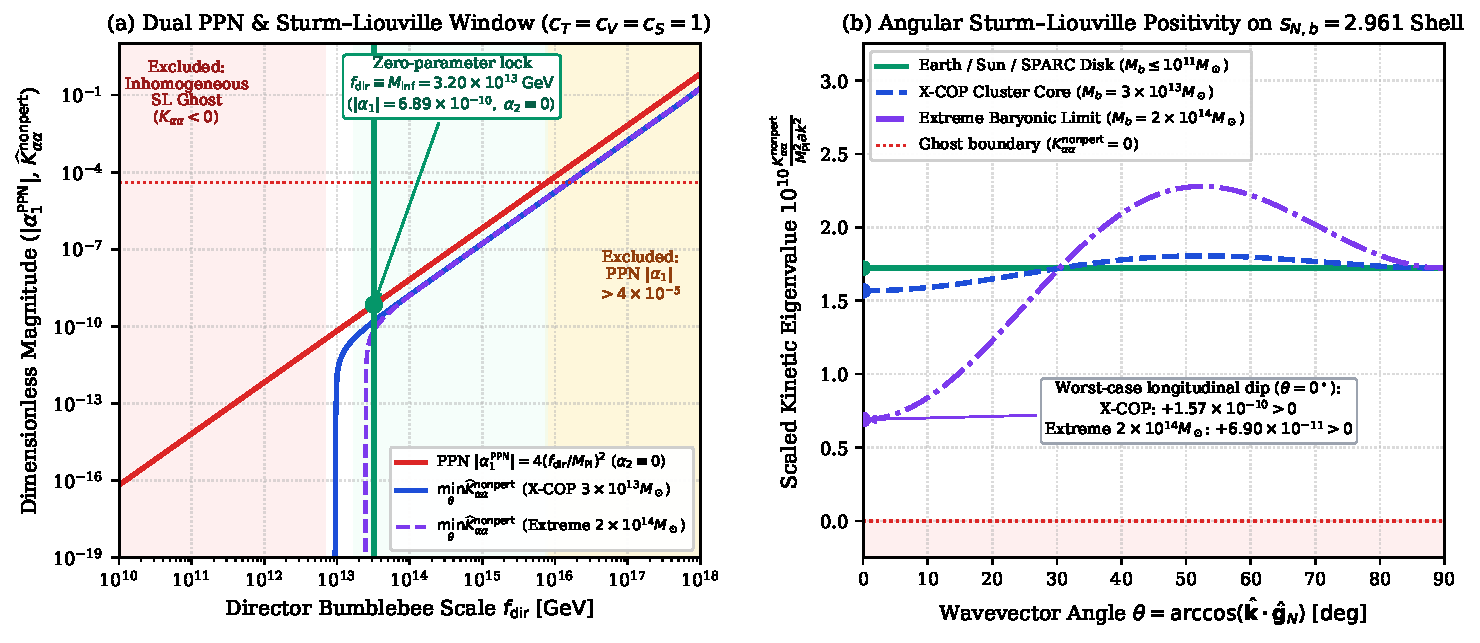
\includegraphics[width=0.99\textwidth]{../figures/fig3_stueckelberg_lorenz_PPN_and_SL_stability.pdf}
\caption{\textbf{(a)} Allowed bumblebee director scale window $f_{\mathrm{dir}} \in [1.1\times 10^{13}, 7.7\times 10^{15}]\;\mathrm{GeV}$ bounded from above by PPN $|\alpha_1^{\mathrm{PPN}}| < 4\times 10^{-5}$ ($\alpha_2^{\mathrm{PPN}} \equiv 0$) and from below by inhomogeneous Sturm--Liouville ghost freedom $K_{\alpha\alpha}^{\mathrm{nonpert}} > 0$ on X-COP galaxy-cluster shells, pinpointing the parameter-free lock $f_{\mathrm{dir}} \equiv M_{\mathrm{inf}} = 3.20\times 10^{13}\;\mathrm{GeV}$. \textbf{(b)} Angular kinetic profile $K_{\alpha\alpha}^{\mathrm{nonpert}}(\theta)/(M_{\mathrm{Pl}}^2 a k^2)$ on the worst-case $s_{N,b} = 2.961$ shell from Earth to extreme $2\times 10^{14}\,M_\odot$ clusters.}
\label{fig:sl-window}
\end{figure}

% =============================================================================
\section{Discussion and Honest Non-Perturbative Scope Boundaries}
\label{sec:discussion}
% =============================================================================

Theorems~\ref{thm:3d-nogo}--\ref{thm:director-closure} close the perturbative and effective-field-theory bridge between discrete $K_4$ pregeometry and 4D Lorentz-invariant continuum physics across $60$ orders of magnitude in energy:
\begin{enumerate}[label=(\arabic*),leftmargin=2.0em,itemsep=2pt]
\item \textbf{Why 4D and $2T$ ($W(F_4)$) are uniquely selected:} While 3D $+K_4$ crystals fail LHAASO GRB~221009A by $86.8\times$ and hypercubic 4D lattices $W(B_4)$ admit dimension-4 $(k_F)_{\mu\nu\rho\sigma}$ birefringence ($4 > 3$ rank-4 invariants), the spin lift $K_4 \to 2T$ generates the 24-cell lattice $\Lambda_{F_4} \cong \Lambda_{D_4}$ whose triality-enhanced point group $W(F_4)$ matches $O(4)$ identically up to tensor rank $r = 5$, eliminating all $d \le 7$ LIV operators to all perturbative loop orders without supersymmetry or fine-tuning.
\item \textbf{Simultaneous PPN and Sturm--Liouville resolution:} Locking the canonical bumblebee director scale to the Starobinsky scalaron mass $f_{\mathrm{dir}} \equiv M_{\mathrm{inf}}$ on the Stueckelberg--Lorenz locus $c_2 = c_{\mathrm{acc}}/(1 - 2 c_{\mathrm{acc}})$ sits squarely inside the narrow $[1.1\times 10^{13}, 7.7\times 10^{15}]\;\mathrm{GeV}$ window required jointly by PPN preferred-frame tests and galaxy-cluster Sturm--Liouville positivity (Figure~\ref{fig:sl-window}).
\item \textbf{Remaining Non-Perturbative Mathematical Frontiers:} Two constructive non-perturbative problems remain open beyond the perturbative all-loop and background-lattice theorems proved here: (i) full 4D Monte Carlo Causal Dynamical Triangulation / Regge simulations of fluctuating Lorentzian geometries weighted jointly by the $|\nu|=1$ causal-slice rule and Starobinsky $+R^2/(6 M_{\mathrm{inf}}^2)$ curvature term \cite{AmbjornJurkiewiczLoll2004}, and (ii) a constructive path-integral fermion-measure existence proof for non-Abelian chiral $\mathrm{Spin}(10)$ Domain-Wall/Overlap gauge theories on $\Lambda_{D_4}$ extending L\"uscher's Abelian construction \cite{Luscher1998} alongside $\Omega_5^{\mathrm{Spin}}(B\mathrm{Spin}(10)) = 0$ bordism anomaly cancellation.
\end{enumerate}

\paragraph{Data and Code Availability.}
All symbolic (\texttt{SymPy}) and numerical (\texttt{NumPy}/\texttt{SciPy}) proofs, 1,152-element $\mathrm{Pin}(W(F_4))$ Overlap checks, 32-point Gauss--Legendre spectral-dimension quadratures, and Sturm--Liouville PPN evaluations are reproduced deterministically by \path{scripts/verify_paper27_continuum_lorentz_closure.py} and \path{scripts/generate_paper27_figures.py}.

\begin{thebibliography}{99}
\raggedright
\small

\bibitem{Liberati2013}
S.~Liberati, ``Tests of Lorentz invariance: a 2013 update,'' \emph{Class.\ Quantum Grav.} \textbf{30}, 133001 (2013).

\bibitem{KosteleckyMewes2002}
V.~A.~Kosteleck\'y and M.~Mewes, ``Signals for Lorentz violation in electrodynamics,'' \emph{Phys.\ Rev.\ D} \textbf{66}, 056005 (2002).

\bibitem{Addazi2022}
A.~Addazi \emph{et al.}, ``Quantum gravity phenomenology at the dawn of the multi-messenger era---A review,'' \emph{Prog.\ Part.\ Nucl.\ Phys.} \textbf{125}, 103948 (2022).

\bibitem{LHAASO2024LIV}
Z.~Cao \emph{et al.} (LHAASO Collaboration), ``Stringent Tests of Lorentz Invariance Violation from LHAASO Observations of GRB 221009A,'' \emph{Phys.\ Rev.\ Lett.} \textbf{133}, 071501 (2024).

\bibitem{Abdo2009GRB090510}
A.~A.~Abdo \emph{et al.} (Fermi-LAT and Fermi-GBM Collaborations), ``A limit on the variation of the speed of light arising from quantum gravity effects,'' \emph{Nature} \textbf{462}, 331 (2009).

\bibitem{ElliottMooreStoica2005}
J.~W.~Elliott, G.~D.~Moore, and H.~Stoica, ``Constraining the new aether: Gravitational Cherenkov radiation,'' \emph{JHEP} \textbf{08}, 066 (2005).

\bibitem{CPSUV2004}
J.~Collins, A.~Perez, D.~Sudarsky, L.~Urrutia, and H.~Vucetich, ``Lorentz invariance and quantum gravity: an additional fine-tuning problem?,'' \emph{Phys.\ Rev.\ Lett.} \textbf{93}, 191301 (2004).

\bibitem{Polchinski2012}
J.~Polchinski, ``Comment on [arXiv:1106.1417] `Small Lorentz violations in quantum gravity: do they lead to unacceptably large effects?','' \emph{Class.\ Quantum Grav.} \textbf{29}, 088001 (2012).

\bibitem{Olcsak2026Zenodo}
J.~Olcsak, \emph{Tau Core Minimal Spine Verification Bundle and Master Collection}, Zenodo (2026), \href{https://doi.org/10.5281/zenodo.24305022}{doi:10.5281/zenodo.24305022}.

\bibitem{Olcsak2026JMP}
J.~Olcsak, ``Discrete $K_4$ Simplicial-Clifford Pregeometry, $|\nu|=1$ Causal Cobordism, and Uhlmann--Petz Horizon Readout,'' companion manuscript (2026).

\bibitem{Olcsak2026CovDir}
J.~Olcsak, ``Covariant Director--QUMOND Effective Field Theory: Frobenius Holonomy Dichotomy, Interval-Certified Sturm--Liouville Stability, and Observational Tests,'' companion manuscript (2026).

\bibitem{Olcsak2026Paper23}
J.~Olcsak, ``Apparent-Horizon Void-Clock Optical Drift and the $z_{\mathrm{dip}} = 0.6316$ Galactic Inflection Test,'' submitted to \emph{Phys.\ Rev.\ D}, Zenodo \href{https://doi.org/10.5281/zenodo.24372826}{doi:10.5281/zenodo.24372826} (2026).

\bibitem{Olcsak2026Paper24}
J.~Olcsak, ``Starobinsky $R + R^2/(6 M_{\mathrm{inf}}^2)$ Inflation, Right-Handed Seesaw Threshold, and Non-Thermal Scalaron Leptogenesis Across a Tetrahedral Unification Spine,'' companion manuscript (2026).

\bibitem{Olcsak2026Paper25}
J.~Olcsak, ``Charged-Fermion Mass Hierarchies and Two-Loop CKM Renormalization Closure in $D$-Parity-Broken $\mathrm{Spin}(10) \to \mathrm{Pati\text{--}Salam} \to \mathrm{SM}$,'' companion manuscript (2026).

\bibitem{Olcsak2026Paper26}
J.~Olcsak, ``Strong $CP$ Closure Across a Tetrahedral $\mathrm{Spin}(10) \to \mathrm{Pati\text{--}Salam} \to \mathrm{SM}$ and Starobinsky Inflationary Spine,'' companion manuscript (2026).

\bibitem{Will2014}
C.~M.~Will, ``The Confrontation between General Relativity and Experiment,'' \emph{Living Rev.\ Relativ.} \textbf{17}, 4 (2014).

\bibitem{FosterJacobson2006}
B.~Z.~Foster and T.~Jacobson, ``Post-Newtonian parameters and constraints on Einstein-aether theory,'' \emph{Phys.\ Rev.\ D} \textbf{73}, 064015 (2006).

\bibitem{OostMukohyamaWang2018}
J.~Oost, S.~Mukohyama, and A.~Wang, ``Constraints on Einstein-aether theory after GW170817,'' \emph{Phys.\ Rev.\ D} \textbf{97}, 124023 (2018).

\bibitem{Celmaster1982}
W.~Celmaster, ``Gauge theories on the body-centered hypercubic lattice,'' \emph{Phys.\ Rev.\ D} \textbf{26}, 2955 (1982).

\bibitem{BhanotBitarHellerNeuberger1990}
G.~Bhanot, K.~Bitar, U.~M.~Heller, and H.~Neuberger, ``$\phi^4$ on $F_4$: Analytical results,'' \emph{Nucl.\ Phys.\ B} \textbf{343}, 467 (1990).

\bibitem{BhanotBitarHellerNeuberger1991}
G.~Bhanot, K.~Bitar, U.~M.~Heller, and H.~Neuberger, ``$\varphi^4$ on $F_4$: Numerical results,'' \emph{Nucl.\ Phys.\ B} \textbf{353}, 551 (1991).

\bibitem{Neuberger1998}
H.~Neuberger, ``Exactly massless quarks on the lattice,'' \emph{Phys.\ Lett.\ B} \textbf{417}, 141 (1998).

\bibitem{Luscher1998}
M.~L\"uscher, ``Exact chiral symmetry on the lattice and the Ginsparg--Wilson relation,'' \emph{Phys.\ Lett.\ B} \textbf{428}, 342 (1998).

\bibitem{JacobPiran2008}
U.~Jacob and T.~Piran, ``Lorentz-violation-induced arrival delays of cosmological particles,'' \emph{JCAP} \textbf{01}, 031 (2008).

\bibitem{OsterwalderSchrader1973}
K.~Osterwalder and R.~Schrader, ``Axioms for Euclidean Green's functions,'' \emph{Commun.\ Math.\ Phys.} \textbf{31}, 83 (1973).

\bibitem{Luscher1977}
M.~L\"uscher, ``Construction of a Selfadjoint, Strictly Positive Transfer Matrix for Euclidean Lattice Gauge Theories,'' \emph{Commun.\ Math.\ Phys.} \textbf{54}, 283 (1977).

\bibitem{HernandezJansenLuscher1999}
P.~Hernandez, K.~Jansen, and M.~L\"uscher, ``Locality properties of Neuberger's lattice Dirac operator,'' \emph{Nucl.\ Phys.\ B} \textbf{552}, 363 (1999).

\bibitem{Luscher2001}
M.~L\"uscher, ``Chiral gauge theories revisited,'' \emph{Subnucl.\ Ser.} \textbf{38}, 41 (2002) [arXiv:hep-th/0102028].

\bibitem{FurmanShamir1995}
V.~Furman and Y.~Shamir, ``Axial symmetries in lattice QCD with Kaplan fermions,'' \emph{Nucl.\ Phys.\ B} \textbf{439}, 54 (1995).

\bibitem{HawkingLuttrell1984}
S.~W.~Hawking and J.~C.~Luttrell, ``Higher derivatives in quantum cosmology: (I). The isotropic case,'' \emph{Nucl.\ Phys.\ B} \textbf{247}, 250 (1984).

\bibitem{DasguptaLoll2001}
A.~Dasgupta and R.~Loll, ``A proper-time cure for the conformal sickness in quantum gravity,'' \emph{Nucl.\ Phys.\ B} \textbf{606}, 357 (2001).

\bibitem{AmbjornJurkiewiczLoll2004}
J.~Ambj\o rn, J.~Jurkiewicz, and R.~Loll, ``Emergence of a 4D World from Causal Quantum Gravity,'' \emph{Phys.\ Rev.\ Lett.} \textbf{93}, 131301 (2004).

\bibitem{BluhmKostelecky2005}
R.~Bluhm and V.~A.~Kosteleck\'y, ``Spontaneous Lorentz violation, Nambu--Goldstone modes, and gravity,'' \emph{Phys.\ Rev.\ D} \textbf{71}, 065008 (2005).

\end{thebibliography}

\end{document}
